\begin{frame}
	\frametitle{Moltres}
	\begin{columns}
		\column[t]{5cm}
		\begin{itemize}
			\item Moltres is an application code built on the \gls{MOOSE}
			framework, for the simulation of \glspl{MSR}.
			\item MOOSE is an open source finite element framework that
			relies on libMesh and PETSc for their advanced meshing and PDE
			solver capabilities.
			\item MOOSE provides a simple interface for creating application
			codes for simulating various physical phenomena.
			\item Moltres can run transient, fully implicit coupled
			neutronics/thermal-hydraulics simulations of \glspl{MSR}.
		\end{itemize}
		\column[t]{5cm}
%		\begin{figure}
%			\centering
%			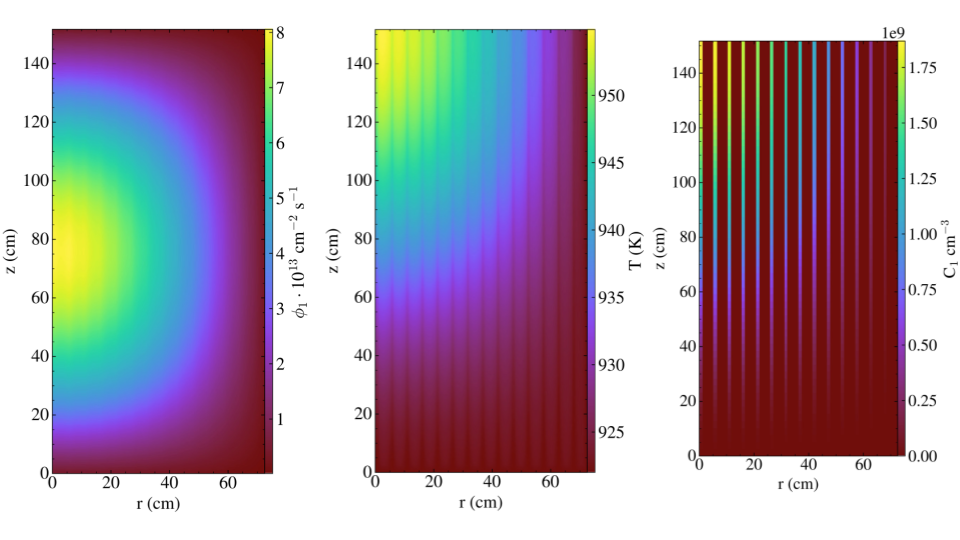
\includegraphics[width=.9\textwidth]{./images/msre}
%		\end{figure}
\end{frame}